\section{Case studies}
\label{sec:case_studies}

After having presented our measurement platform and parameters, built on top of
Atlas, we now evaluate it by discussing two cases of large-scale
restrictions on online content and social media platforms.  In particular, Turkey's ban on social media platforms in
Section~\ref{sec:turkey} and Russia's filtering of opposition LiveJournal content in Section~\ref{sec:russia}. All dates and times reported follow Coordinated Universal Time.

% *** Can I try to negotiate with all dir authorities?

\subsection{Turkey's ban of Twitter}
\label{sec:turkey}

In late March, social media users began to report limitations on the
availability of Twitter across the Turkey's Internet Service Providers.
YouTube and Twitter had both become the target of condemnation by Prime Minister
Erdogan in preceding months. By March 20, the Turkish government's Information
and Communication Technologies Authority (BTK) mandated the filtering of
Twitter across the country's service providers.

Turkey's Internet filtering has previously been characterized as DNS tampering and
IP blocking \cite{akdeniz2010report}, which both fall under the measurements
possible through Atlas.  Upon news of the Twitter ban, we
scheduled hourly measurements of local DNS answers, SSL connectivity, and
Traceroute reachability for Twitter, YouTube, Google Public DNS and the Tor
Project through ten probes, covering nine ASNs.  The selected measurement targets sought to longitudinally
document the Turkish government's disruption of controversial political
content, identified based statements by authorities and potential usefulness for
circumventing information controls. Seeking to address an immediate interest for real-time
awareness, the measurements did not attempt to assess the whole of Turkey's content
restrictions. As illustrated in Figure~\ref{image:tr-social_media_filtering}, we
found at least six shifts in content restrictions and blocking strategies
within a two week period.

\begin{figure*}
  \centering
  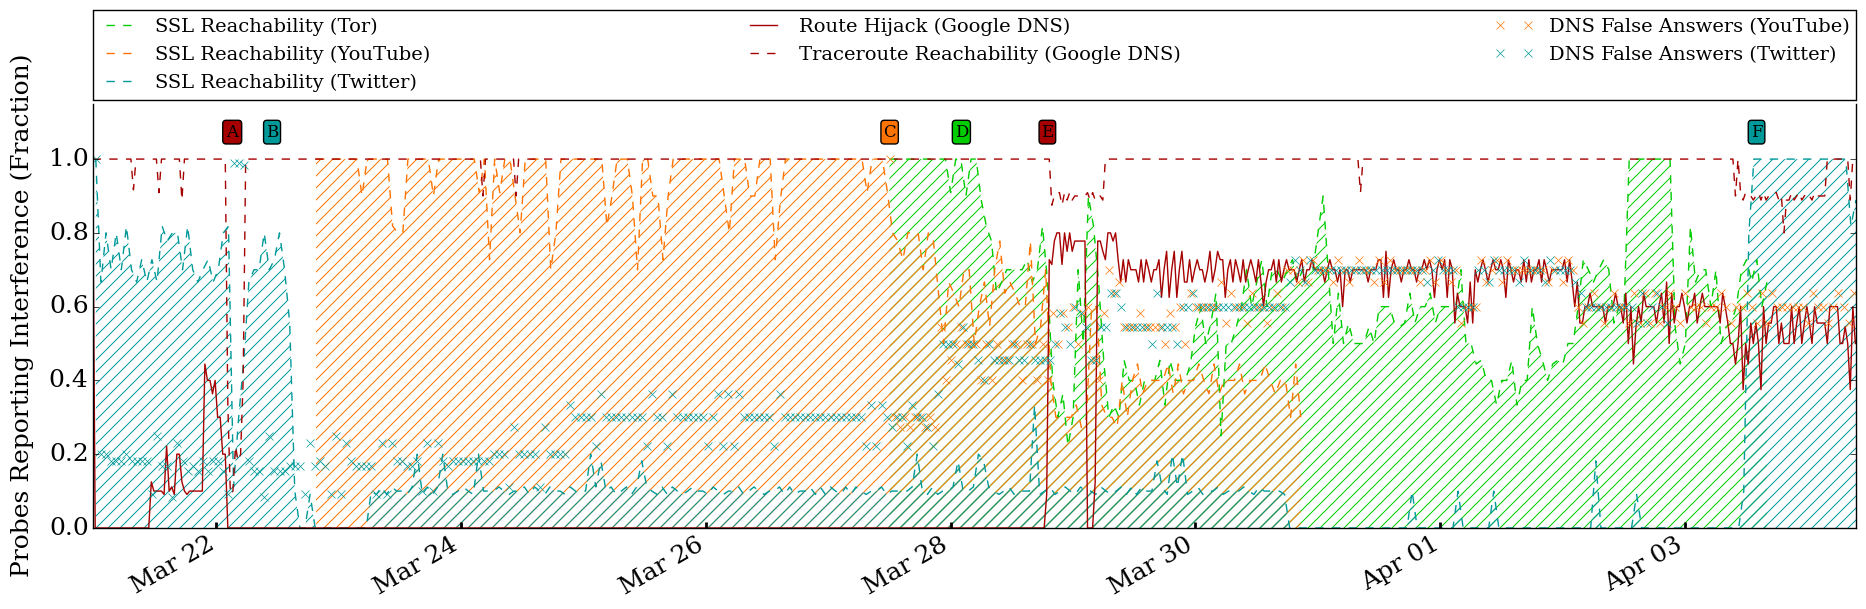
\includegraphics[width=0.9\textwidth]{diagrams/tr-20140321-20140407-social_media_filtering.png}
  \caption{Disruption of Social Media Platforms in Turkey, March -- April 2014}
  \label{image:tr-social_media_filtering}
\end{figure*}


While the BTK and compliant ISPs rely on DNS manipulation and IP blocking, it
appears that the former is more popular.  As of April 24, 2014, the
Turkish-language anti-censorship site \textit{Engelliweb}, which tracks
blocked content, only lists 167 IP addresses restricted in
country, compared to 40,566 domain names \cite{engelliweb}.
% The popularity of content distribution networks
% and shared hosting easily makes address-based blocking either overbroad,
% creating collateral damage from restricting all domains and content on a shared
% host, or inefficiently narrow. Iranian authorities reportedly faced an aspect
% of this in October 2012, when an attempt to block  YouTube was blamed for
% week-long disruptions on access to Gmail, likely a result of shared
% infrastructure and addresses across Google's services \cite{bbc2012gmail}.
In absence of address blocking or HTTP filtering, users that received valid DNS
answers for Twitter's domain names could browse without further interference.
As a result, foreign DNS servers quickly became both a circumvention mechanism
and a political statement, with the addresses of alternative services offered
by Google and OpenDNS reportedly graffitied across the the country in protest
of the ban.

% The ease and rate that users were appeared to be bypassing the filters, by some
% indications more tweets were sent after the restrictions than before, prompted
% broader crackdown by authorities.
On the morning of March 22nd (see Figure~\ref{image:tr-social_media_filtering},
\textbf{Event A}), between 01:00 and 02:00, backbone providers Tellcom \.{I}leti\c{s}im
Hizmetleri and Turk Telekom began disrupting Google's Public DNS service
through the IP blocking of its two prominent addresses (8.8.8.8 and 8.8.4.4).
% This restriction would have disrupted access to filtered and non-filtered sites
% alike through interfering with the translation of names to Internet-routable
% addresses. Use of Google's DNS is commonplace in the country, and not
% necessarily indicative of an intent to circumvent filters. By some metrics
% 18.3\% of Internet users in Turkey rely on Google Public DNS
% \cite{ispcolumn2013googledns}. Given this cost, within hours,
By 06:00 the same morning, the DNS blocking had been removed across all ISPs.
Instead, to buttress the restrictions, providers shortly began to drop all
outgoing traffic to addresses associated with the twitter.com domain,
regardless of port or provider (\textbf{Event B}). By 16:00 of that
day, no Atlas probe could directly negotiate an SSL connection with Twitter
until the removal of the ban nearly two weeks later.

On March 27 (\textbf{Event C}), after recordings were posted of Turkish
national security officials discussing possible military action against Syria,
YouTube was blocked through false DNS answers for the youtube.com domain.
Within the Atlas network, this restriction appears as a slow decline in the
number of probes able to establish a connection to the platform. However, unlike Twitter, a
significant minority of probes remained able to communicate with YouTube.
Google's intertwined infrastructure presents risk of collateral damage with network prefix restrictions, which were not
present with Twitter. Thus, clients that were able to receive a valid address could reliably bypass the ban.

% Although the BTK is alleged to have ordered the installation of deep packet
% inspection equipment for purposes of lawful interception and censorship
% \cite{kirlidog2011deep}, restrictions on circumvention and anonymizations tools
% appear to have been limited to the filtering of services' websites.
Beginning
March 28, Atlas probes in-country began to fail to establish an SSL
connections to torproject.org (\textbf{Event D}). However, this restriction
neither included IP restrictions, nor was there evidence of interference with
the accessibility of the network. Atlas probes could continue to negotiate
valid connections to Tor's Directory Authories. Throughout the increased
manipulation of local DNS services, nearly half of the Atlas probes remained
connected due to their use of foreign DNS services.
% More aggressive
% restrictions were perhaps inevitable due to international attention on the
% rapid adoption of circumvention tools and Google Public DNS as an indicator of
% the futility of the ban.

Later in the evening, March 28, hosts querying foreign-based DNS servers began to
receive the same false answers as those provided domestically, leading to a
rapid drop in availability of YouTube and Tor (\textbf{Event E}). A
publicly-available traceroute scheduled by third-parties on the Atlas network 
against Google Public DNS returned idiosyncratic and
spontaneous shifts in Turkey's network topology timed with these
changes. This appears within traceroutes as a shortening in the
number of hops to Google, with a multifold reduction in traffic latency and the
absence of international hosts in path. The core telecommunications provider
Turk Telekom had begun to reroute traffic destined for Google to a local DNS
server. Only TEKNOTEL Telekom maintained
consistently valid routes for Google, through Telecom Italia
Sparkle. However, two days later Doruk \.{I}leti\c{s}im and Net Elektronik
Tasar{\i}m reestablished connectivity through Euroweb Romania, circumventing upstream interference. Turk Telekom's redirection was finally removed late on April 7.

By April 3th, despite continued hijacking of Google Public DNS and interference with YouTube, Twitter was unblocked for all probes
(\textbf{Event F}).

\begin{table}
    \begin{tabular}{l | c | c | c | c}
        \textbf{Target} & \textbf{Type}  & \textbf{Probes}  & \textbf{Freq (s)}  & \textbf{Credits}\\
        \hline
		 Twitter & SSL & 10 & 3600 & 2400 \\
		 YouTube & SSL & 10 & 3600 & 2400 \\
		 Tor & SSL & 10 & 3600 & 2400 \\
		 Twitter & DNS (U) & 10 & 3600 & 2400 \\
		 YouTube & DNS (U) & 10 & 3600 & 2400 \\
		 Twitter & Tracert & 10 & 3600 & 7200 \\
        \hline
        \multicolumn{4}{l}{\textit{Total (Daily)}}  & 19200\\
        \multicolumn{4}{l}{\textit{Probes Required}} & 0.89\\
        \hline        
    \end{tabular}
    \caption{Cost of Measurements for Section~\ref{sec:turkey}}
    \label{table:tr-costs}
\end{table}

% % % % % % % % % % % % % % % % % % % % % % % % % % % % % % % % % % % % % % % %
\subsection{Private sector cooperation in Russian filtering of Alexei Navalny}
\label{sec:russia}
% % % % % % % % % % % % % % % % % % % % % % % % % % % % % % % % % % % % % % % %

% Concurrent to broader restrictions on independent media, on March 13, 2014,
% Russia's Federal Service for Supervision in the Sphere of Telecom, Information
% Technologies and Mass Communications (Roskomnadzor) announced the blacklisting
% of opposition figure Alexei Navalny's LiveJournal blog, due to claimed
% violations of the terms of his house arrest. Shortly after the order was
% issued, Russian social media and state news agencies reported that access to
% the entirity of LiveJournal had been temporarily disrupted on some Interent
% providers due to their inability to distinguish traffic to different blogs
% within the site \cite{itar2014livejournal}. Overblocking has proven a recurrent
% issue in Russia. When a regional ISP, Netis Telekom, previously blocked the
% full site while complying with a court order against a neo-nazi blog,
% LiveJournal's Russian Director Ilya Dronov attributed the event to several
% ISPs' reliance on IP-based filtering and the inclusion of IP addresses within
% court orders \cite{leta2012livejoural}. 

On March 13, 2014, Russia's Federal Service for Supervision in the Sphere of Telecom, Information Technologies and Mass Communications (Roskomnadzor) ordered the blacklisting of opposition figure Alexei Navalny's LiveJournal blog.

% At the same time as Navalny's censorship, four opposition news portals were
% filtered based on the allegations that they called for ``illegal activity and
% participation in mass events that are conducted contrary to the established
% order,'' including grani.ru \cite{ibtimes2014russia}. As with Turkey, Russia's
% content restrictions have previously been attributed to DNS poisoning and IP
% filtering, presenting the same potential circumvention strategies and
% measurement opportunities \cite{rugovdns, verkamp2012inferring}. However, with
% a random sample of 255 probes across 147 ASNs in Russia, only 38 probes on 20
% ASNs received aberrant DNS answers. Within this subset, probes received a
% diverse, consistent selection of ten unique addresses, including two within
% RFC1918, private network address space (10.52.34.222 and 192.168.103.162). A
% greater selection, 40 probes across 23 ASNs, of traceroutes to the port 80 for
% the primary address associated with Grani as of April 30 (23.253.120.92) failed
% within Russia network space. Based on Russian filtering documentation efforts,
% the order that restricted Grani identifies at least fourteen addresses
% connected with the site \cite{antizapret2014}. An additional address that
% appears in the Grani order was found blocked on 36 probes and 22 ASNs,
% highlighting inconsistency in implementation and upkeep.
At the same time, independent media portals were filtered, including the news site
grani.ru~\cite{ibtimes2014russia}.  Similar to Turkey, Internet filtering in
Russia is frequently conducted by IP blocking and DNS
poisoning~\cite{rugovdns,verkamp2012inferring}.  However, with a random sample
of 255 probes across 147 ASNs in Russia, only 38 probes on 20 ASNs received
aberrant DNS answers for Grani. Within this subset, probes received a diverse, consistent
selection of \emph{ten unique addresses}, including two within RFC1918, private
network address space (10.52.34.222 and 192.168.103.162). A greater selection,
40 probes across 23 ASNs, of traceroutes to the port 80 for the primary address
associated with Grani as of April 30 (23.253.120.92) failed within Russia
network space. 

In contrast to Grani, a locally-resolved DNS query for navalny.livejournal.com
over 255 probes on 146 ASNs received a consistent reply of 208.93.0.190, which
matched answers internationally with only one anomalous response, a formerly valid
address. The blocking of Navalny's blog must be different from Grani. While the
returned DNS A record of 208.93.0.190 falls within a network prefix owned by
LiveJournal Inc. (208.93.0.0/22), over the 1462 LiveJournal subdomains in
Alexa's Top 1 million list, 1450 blogs resolved to another address, 208.93.0.150.
Based on requests made independently of the Atlas network from Europe, both hosts appear to be front servers for the LiveJournal platform, as they return
the same SSL Certificate and content. Requests to 208.93.0.150
with a HTTP Host header set to navalny.livejournal.com retrieves the correct
content, and non-blacklisted content is retrievable through 208.93.0.190.

As of April 2014, only five subdomains on livejournal.com could be found whose
DNS A records resolved to the address 208.93.0.190, Table
\ref{table:lj-blocked-blogs}, four of which are listed within Alexa's top sites. All
the blogs found on this alternative host have been publicly declared by Russian
authorities as in violation the country's media laws for promotion of political
activities or extremism, and two are listed within publicly-available filter
site lists. 

\begin{figure*}
  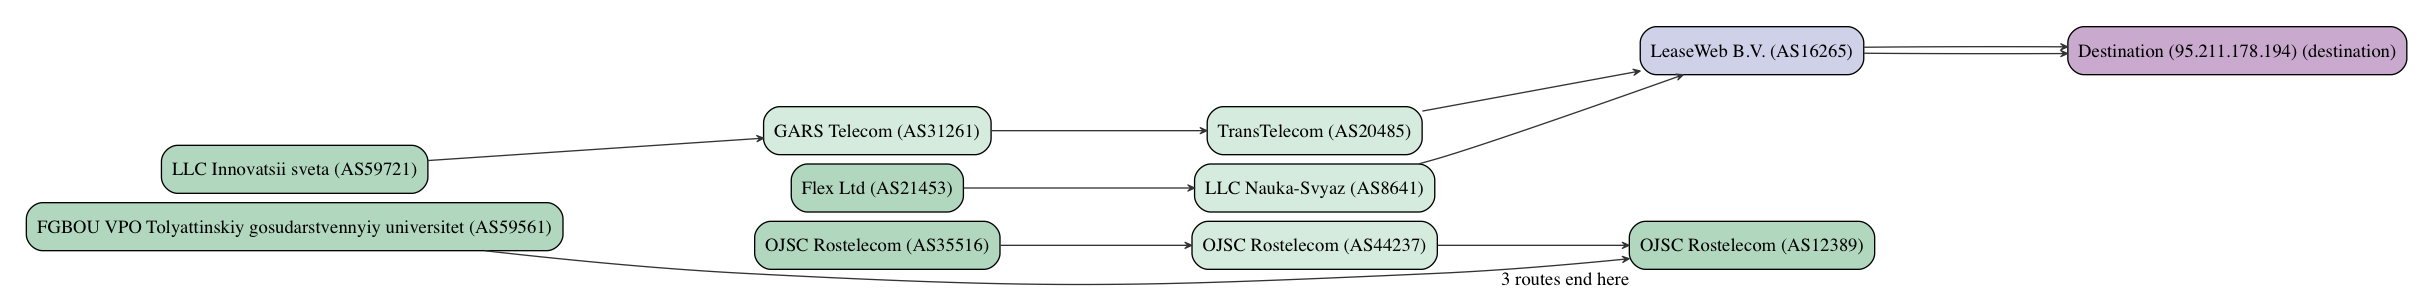
\includegraphics[width=\textwidth]{diagrams/atlas_cache-results-measurement_id-1663748.png}
  \caption{Rostelecom (AS12389) Hijack of grani.ru Traffic, April 30 2014}
  \label{image:ru-grani-hijack}
\end{figure*}

Based on timing, filtering lists, available domain names records,
and Atlas network measurements, it appears that a host was specially-established 
to faciliate Russian restrictions on content within the LiveJournal platform. 
Using HTTPS Ecosystem Scans as a metric of accessibility
\cite{projectsonar}, the LiveJournal frontend at 208.93.0.190 came online
between February 10 and February 17, with the address otherwise unused until
then. Two months later, the Ukrainian LiveJournal blog `Pauluskp'
(pauluskp.livejournal.com), which had covered Russian involvement in Crimea,
was filtered with the administrative order listing an IP Address of
208.93.0.190. However, as recently as six days before, the blog was recorded as
pointing to the main LiveJournal host. Similarly, the movement of Navalny's
blog was noticed within social media \cite{miptru2014}. It appears that in the
lead up to or at the time of filtering orders, LiveJournal coordinates with
authorities to alter the DNS A record for blogs designated by Roskomnadzor, in
order to segregate blacklisted content from the rest of the platform.

\begin{table}
    \begin{tabular}{l | c | c}
        \textbf{Subdomain} & \textbf{Language} & \textbf{Roskomnadzor}\\
        \hline
        drugoi-nnover & Russian & Yes\\
        m-athanasios & Russian & Yes\\
        imperialcommiss & Russian & Yes\\
        pauluskp & Russian & Yes \\
        navalny & Russian & Yes \\
        \hline
    \end{tabular}
    \caption{LiveJournal DNS A Records of 208.93.0.190}
    \label{table:lj-blocked-blogs}
\end{table}

Segregated LiveJournal content and blacklisted addresses are subject to an
additional, unknown method of network-layer interception performed within the
backbone network of Rostelecom (AS12389). While blog content is not
accessible over HTTPS, frontend hosts for LiveJournal offer SSL services for the purpose of
securing the transmission of user credentials. On April 28, 78 of 343 Russian
probes returned either irregular responses or failed to connect to the alternative LiveJournal host by address, of which 40
probes on 29 ASNs returned SSL certificates with common name or locations
fields attributed to Russian ISPs. Based on HTTPS data, the four aberrant
certificates captured have been seen previously on seven Russian addresses
belonging to the State Institute of Information Technologies, Rostelecom and
Electron telecom network. Three of these hosts are responsive and still match
certificates, two are generic ISP homepages and one notifies of the blocking of
the site `rutracker.ru.' Other measurements that are unresponsive could be
indicative of port blocking by other intermediaries or the redirection of
traffic to a server that is not listening for SSL connections.

The invalid certificates indicate that an intermediary in transit has
redirected the traffic out of its expected path to a third-party
server controlled by Russian entities. This approach is different from the
normal man-in-the-middle injection of responses seen in countries such as Iran and Syria, and
ellucidates the potential for Russian ISPs to falsify content or gather user
credentials. The observed behavior is not limited to protocol or port, although the end
host appears to be only responsive to TCP requests,
Figure~\ref{image:ru-grani-hijack}. This holistic interference across Rostelecom's downstream peers suggests
redirection at the network layer, rather than application-based classification of traffic associated with deep packet inspection. Moreover,
adjacent addresses within the same network, such as the normal frontend for
LiveJournal, traverse a valid international path. Instead, blacklisted traffic
appears to be coerced into a path controlled by Rostelecom, indicating a narrowly-crafted interference with
normal routing through false advertisements or forwarding.
